\documentclass[a4paper]{scrreprt}

\usepackage[german]{babel}
\usepackage[utf8]{inputenc}
\usepackage[T1]{fontenc}
\usepackage[titletoc]{appendix}
\usepackage{ae}
\usepackage{enumitem}
\usepackage[bookmarks,bookmarksnumbered]{hyperref}
\usepackage{graphicx}
\usepackage{array}
\usepackage{morefloats}
\usepackage{calc}

%Preambel texdoclet
\usepackage{color}
\usepackage{ifthen}
\usepackage{makeidx}
\usepackage{ifpdf}
\usepackage[headings]{fullpage}
\usepackage{listings}
\lstset{language=Java,breaklines=true}
\DeclareOldFontCommand{\bf}{\normalfont\bfseries}{\mathbf}

\newcommand{\entityintro}[3]{%
  \hbox to \hsize{%
    \vbox{%
      \hbox to .2in{}%
    }%
    {\bf  #1}%
    \dotfill \pageref{#2}%
  }
  \makebox[\hsize]{%
    \parbox{.4in}{}%
    \parbox[l]{5in}{%
      \vspace{1mm}%
      #3%
      \vspace{1mm}%
    }%
  }%
}
\newcommand{\refdefined}[1]{
\expandafter\ifx\csname r@#1\endcsname\relax
\relax\else
{$($in \ref{#1}, page \pageref{#1}$)$}\fi}
%\date{null}
\chardef\textbackslash=`\\
%\makeindex

\bibliographystyle{plain}
\graphicspath{{resourcen/}}

%Used for including MetaUML diagrams
%\usepackage{emp}
%\usepackage{ifpdf}
%\ifpdf
\DeclareGraphicsRule{.1}{mps}{*}{}
%\fi

\makeatletter
\def\namedlabel#1#2{\begingroup
   \def\@currentlabel{#2}%
   \phantomsection#2\label{#1}\endgroup
}
\makeatother
% Inhaltsverzeichnis Ebenen definieren, zB bis zu Subsection
\setcounter{secnumdepth}{4}
\setcounter{tocdepth}{1}

\usepackage[toc,acronym]{glossaries}

\usepackage{xparse}

\makeatother
\begin{document}

\title{Implementierung\\
Graph von Ansicht}
\date{}
\author{Nicolas Boltz   \\ uweaw@student.kit.edu
  \and Jonas Fehrenbach \\ urdtk@student.kit.edu
  \and Sven Kummetz     \\ kummetz.sven@gmail.com
  \and Jonas Meier      \\ Meierjonas96@web.de
  \and Lucas Steinmann  \\ ucemp@student.kit.edu
}

\titlehead{
\includegraphics[width=150pt]{resourcen/GAns.png}}

\maketitle

% Same
%\begin{abstract}
%\end{abstract}
{\small\tableofcontents}

\chapter{Einleitung}
\label{ch:einleitung}

\chapter{Änderungen am Entwurf}
\label{ch:aenderungen}
%In tabellenform bringen damit einheitlich gelayouted wird

\newcounter{cnr}

\newcommand\change[2]{\textbf{\arabic{cnr}}\addtocounter{cnr}{1}. & \textbf{Aktion:} & #1 \\ & \textbf{Grund:} & #2 \\ [1ex] }
	
\subsection{Gerneral:}
\setcounter{cnr}{1}

\begin{tabular}{llp{0.9\linewidth}}
	\change	{Rename: GraphMLImporter -> GraphmlImporter} 
			{Match Conventions (no more than 1 capital letter in abreviations)}
	\change	{Added Generics to Raw-Types: VertexFilter and EdgeFilter} 
			{Create more type-safety during compile-time.}
	\change	{Moved method getGraphBuilder from IVertexBuilder to IGraphBuilder} 
			{Better possibility to build hierarchical graphs dynamically}
	\change	{Collabsable Graph Interface hinzugefügt} 
			{unterscheiden zwischen einem compoundgraph(z.B. FieldAccess) und einem normalen zusammengeklappten subgraphen}
	\change	{JoanaBuilder Abhängigkeiten hinzugefügt} 
			{Damit jeder Builder weiß von wem er erstellt wurde und sein Produkt bei diesem platzieren kann.}
	\change	{Added AbstractPluginBase} 
			{Many functions in the concrete Plugins are nearly empty, but have to be overwritten. An AbstractPluginBase reduces identical code.}
	\change	{Removed build() functions from IGraphBuilder, IVertexBuilder, IEdgeBuilder.} 
			{build() is now only called on IGraphModelBuilder, which then calls recursively the specific build functions of the concrete classes. (Lucas)}
	\change	{Replaced nodeKind (String) field from JoanaVertex with enum. Adapted interface of JoanaVertex accordingly.} 
			{All reason why using enum is better when possibility are known at compile-time.  (Lucas)}
	\change	{Replaced edgeKind (String) field from JoanaEdge with enum. Adapted interface of JoanaEdge accordingly.} 
			{All reason why using enum is better when possibility are known at compile-time.  (Lucas)}
	\change	{SerializedGraph verschoben. Die View wird nun serialized und nicht das model} 
			{View besitzt mehr Information über den Graphen wie Koordinaten -> wichtig für SvgExporter (Jonas F)}
	\change	{Added class DefaultDirectedEdge and changed DirectedEdge from class to interface. Changed occurences of DirectedEdge to DefaultDirectedEdge in most cases in whole project.} 
			{There was a need of an interface of DirectedEdge (Jonas M)}		
\end{tabular}

\subsection{Sugiyama:}
\setcounter{cnr}{1}

\begin{tabular}{llp{0.9\linewidth}}
	\change	{Changed method return type of reverseEdge(SugiyamaEdge edge) in ICycleRemoverGraph from Set<SugiyamaEdge> to void} 
			{Not really necessary to know which edges have been turned, it can be queried from the edge throug an instance of a SugiyamaGraph (Jonas M)}
	\change	{Added Interface ISugiyamaVertex and let SugiyamaVertex and DummyVertex implement it. Changed every occurence of SugiyamaVertex to ISugiyamaVertex in package sugiyama} 
			{It's necessary to treat SugiyamaVertex and DummyVertex the same way in a common list (Jonas M)}
	\change	{Moved class Point to from package sugiyama to package edu.kit.student.util} 
			{For a better overview (Lucas)}
	\change	{SupplementPath does not extends DirectedEdge anymore.} 
			{?}
\end{tabular}



\chapter{Implementierte Muss- und Wunschkriterien}
\label{ch:implkrit}

\section{Pflichtkriterien}

\subsection{Allgemein}
\begin{itemize}
	\item Anzeige von Graphen (/FA010/)
	\item Anzeige von geschachtelten Graphen (/FA020/)
		\begin{itemize}
			\item Öffnen eines geschachtelten Graphen über ein Kontextmenü eines Knoten wurde nicht implementiert (z.B. Callgraph)
			\item Tastenkürzel existiert nicht
		\end{itemize}
	\item Graphen layouten (/FA030/)
		\begin{itemize}
			\item Constraints für den Methodengraphen werden gesetzt, jedoch nicht im Layout-Algorithmus beachtet.
		\end{itemize}
	\item Knoten und Kanten filtern (/FA040/)
	\item Anwendung einer Arbeitsumgebung (/FA050/)
		\begin{itemize}
			\item CallgraphLayout wird nicht automatisch ausgewählt
		\end{itemize}
	\item Kollabieren von Subgraphen (/FA060/)
		\begin{itemize}
			\item Der Graph wird automatisch neugeladen und ist nicht optional
		\end{itemize}
	\item Ausklappen von kollabierten Subgraphen (/FA070/)
		\begin{itemize}
			\item Der Graph wird automatisch neugeladen und ist nicht optional
		\end{itemize}
\end{itemize}

\subsection{Input/Output}
\begin{itemize}
	\item Graph aus Datei importieren (/FA100/)
		\begin{itemize}
			\item Werden auch generische GraphML Dateien importiert?
		\end{itemize}
	\item Export als Bilddatei (/FA110/)
\end{itemize}

\subsection{Steuerung}
\label{implkrit:steuerung}
\begin{itemize}
	\item Sichtfeld verschieben (/FA200/)
		\begin{itemize}
			\item Die im Pflichtenheft definierte Maustastenbelegung kann von Java leider nicht unter jedem Betriebssystem realisiert werden. Im Fall von Windows 8.1 gibt es eine Funktionalität, die auf den Klick des Mausrads reagiert. Aus diesem Grund wurde die Tastenbelegung leicht abgeändert
			\item Das Sichtfeld verschiebt man nun durch das Drücken von STRG und klicken und ziehen der rechten Maustaste
		\end{itemize}
	\item Zoom-Grad ändern (/FA210/)
		\begin{itemize}
			\item Es existiert kein Fehlschlag (kein Maximum oder Minimum des Zooms
		\end{itemize}
	\item Knoten selektieren (/FA220/) und deselektieren (/FA230/)
		\begin{itemize}
			\item Um das Selektieren und Deselektieren von Knoten benutzerfreundlicher zu gestalten, wurde die Tastenbelegung an die der gängigen Dateisystemexplorer angepasst:
			\item Zum Hinzufügen oder Entfernen eines einzelnen Knotens aus der Selektion von mehreren Knoten muss beim Klicken STRG gehalten werden. Ansonsten wird die komplette Selektion aufgehoben und nur der angeklickte Knoten selektiert.
			\item Ist eine Menge von Knoten selektiert, STRG gedrückt und man selektiert durch ziehen der Maus mehrere Knoten, werden bereits selektierte Knoten aus der Menge entfernt und nicht selektierte Knoten hinzugefügt.
		\end{itemize}
	\item Knoten einer Gruppe hinzufügen (/FA240/)
	\item Gruppe löschen
		\begin{itemize}
			\item Gruppe kann nicht über Kontextmenü gelöscht werden
		\end{itemize}
	\item Wechsel zwischen Graphen (/FA260/)
	\item Informationsanzeige zu einzelnen Knoten und Kanten (/FA270/)
		\begin{itemize}
			\item Keine Informationsanzeige zu Kanten
		\end{itemize}
	\item Statistiken zu Graphen (/FA280/)
	\item Kontextmenü (/FA290/)
\end{itemize}

%Eventuell anders reinbringen
\subsection{Nichtfunktionale Anforderungen}
\begin{itemize}
	%TODO: richtige Formulierung? nicht dass Snelting wieder daran hängen bleibt
	\item Es werden mindestens Graphen mit bis zu 1000 Knoten unterstützt (/NFA010/)
	\item Es werden mindestens Graphdateien mit bis zu 100.000 Knoten insgesamt unterstützt (/NFA020/).. stimmt das?
	\item Die maximale unterstützte Kantenanzahl pro Graph entspricht mindestens der 3-4 fachen Knotenzahl aus /NFA010/ und /NFA020/. (/NFA030/).. stimmt das?
	\item Der Algorithmus, welcher das Graphlayout berechnet ist einfach auswechselbar (/NFA040/)
	%TODO: welche heuristische Methode?
	\item Durch heuristische Methoden wird ein möglichst optimales Ergebnis bei der Einhaltung gegebener Constraints erreicht (/NFA050/) FALSCH!!!
	\item Ein einfacher Sprachwechsel der GUI soll möglich sein (/NFA100/)
		\begin{itemize}
			\item Da Nicolas schlecht implementiert hat ist das nicht möglich
		\end{itemize}
	\item Falls das Programm mit falschen Parametern über die Kommandozeile gestartet wird, soll das Programm nicht abstürzen (/NFA110/)
		\begin{itemize}
			\item Abfangen des Errors wurde aus Zeitgründen in die Testphase verschoben
		\end{itemize}
\end{itemize}

\subsection{Plugins}
\begin{itemize}
	\item Schnittstellen für Plugins in den Bereichen Import, Export, Layoutalgorithmen, Filter für Knoten- und Kantentypen und weitere Operationen auf einzelne Knoten und Kanten (Pflichtenheft Kapitel 7)
	\item Es gibt ein Pluginmanagement-System, welches externe Plugins laden und verwalten kann. (Pflichtenheft Kapitel 7)
\end{itemize}

\subsection{Sonstiges}
\label{implkrit:sonstiges}
\begin{itemize}
	\item Gesetzte Einstellungen (z.B. Speicherort der zueltzt exportierten Datei oder Größe des Fensters) werden gespeichert
		\begin{itemize}
			\item Wurde nicht implementiert
		\end{itemize}
	\item Akzeptieren von Kommandozeilenargumenten
		\begin{itemize}
			\item Das Eingabeformat der Kommandozeilenargumente hat sich zum Pflichtenheft geändert, um ein einfacheres parsen der Parameter zu  ermöglichen. Argumente werden nun im folgenden Format eingegeben: \glqq- -in=<datei>\grqq
		\end{itemize}
	\item Das Produkt wird unter einer freien Lizenz veröffentlicht	
\end{itemize}

\section{Wunschkriterien}
Aus den Wunschkriterien die im Pflichtenheft definiert wurden, wurden aus Zeitmangel keine Implementiert.


\chapter{Implementierungsplan}
\label{ch:implplan}
Um einen Implementierungsplan aufzustellen, wurde das Projekt zuerst anhand der einzelnen Plugins/Pakete aufgeteilt. Danach wurden die Plugins/Pakete noch feiner unterteilt und es wurde versucht einzelne, möglichst voneinander unabhängige, Aufgaben zu finden. Der nötige Arbeitsaufwand zum Bearbeiten der einzelnen Aufgaben wurden von allen Projektmitgliedern abgeschätzt und der Mittelwert als geplante Bearbeitungsdauer festgesetzt. Anhand von den bestehenden Abhängigkeiten der Aufgaben untereinander und der vorausgesetzten wöchentlichen Arbeitsleistung, wurden die Aufgaben auf die einzelnen Wochen und Personen verteilt. \\
\begin{figure}[!htbp]
	\centering
	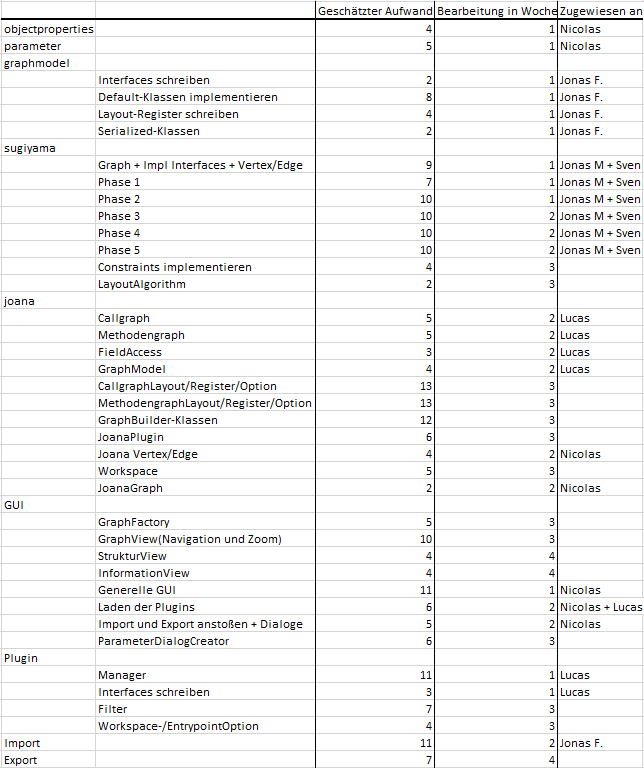
\includegraphics[width=300pt]{week_zero_table.PNG}
	\caption{Erster Implementierungsplan}
	\label{fig:week_zero_table}
\end{figure}

\newpage

\section{Woche 1}
In der ersten Woche wurde der zuerst erstellte Implementierungsplan jedoch komplett überarbeitet. Dies war nötig da im ersten Plan viele Abhängigkeiten zwischen den Aufgaben nicht berücksichtigt wurden. Zum Beispiel hing das restliche Projekt komplett von der Fertigstellung des Sugiyama ab und hätte ohne diesen nicht getestet werden können. Um dieses Problem zu lösen, wurden vorläufige Mockups für die einzelnen Phasen eingeplant. Die anderen Aufgaben wurden zusätzlich in der Abarbeitungsreihenfolge umsortiert, verfeinert und für die ersten zwei Wochen bereits einzelnen Personen zugewiesen. Außerdem wurde eine Excel Tabelle mit dem bereits existierenden Plan erstellt und durch eine Fortschrittsspalte erweitert. In der Fortschrittspalte sollten die Entwickler den prozentualen Fortschritt an den ihnen zugeteilten Aufgaben eintragen. Dadurch konnte ein Fortschrittsdiagram erstellt werden, welchen den aktuellen Soll- und Ist-Zustand des gesamten Projekt visualisiert.\\
\\
Zusätzlich zur Änderung des Plans wurde eine grobe Projektstruktur in Gradle aufgebaut und die bereits im Entwurf erstellte Interfaces in das Projekt überführt. Um die Gradle Projektkonfiguration zu testen wurde eine grobe GUI implementiert und mit der Implementierung der Allgemein genutzten Klassen aus dem Paket "graphmodel"  begonnen.
\begin{figure}[!htbp]
	\centering
	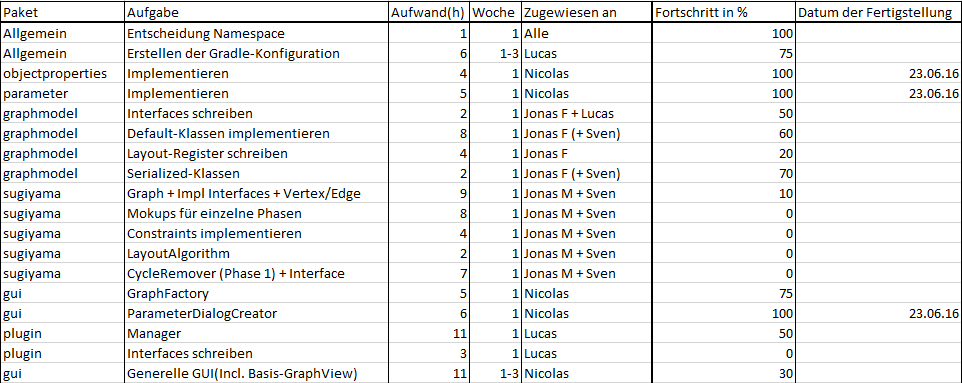
\includegraphics[width=380pt]{week_one_table.PNG}
	\caption{Überarbeiteter Plan für Woche 1 mit Fortschritt}
	\label{fig:week_one_table}
\end{figure}
\subsection{Verzögerungen}
Wie man in \ref{fig:week_one_diagram} sehen kann, hing das Projekt nach der ersten Woche bereits ca. 35 Stunden hinter dem geplanten Zustand hinterher.
Dies lag neben der Tatsache, dass die erste Hälfte der Woche aufgrund von Erschöpfung aus der Entwurfsphase, weniger gearbeitet wurde, als auch daran, dass das Team, welches für die Implementierung des Sugiyama-Layoutalgorithmus eingeteilt wurde, relativ schnell auf konzeptionelle Probleme mit dem im Entwurf definierten Aufbau des SugiyamaGraphen und dessen Kanten/Knoten stieß(siehe \ref{sec:change_sugiyama}).
\begin{figure}[!htbp]
	\centering
	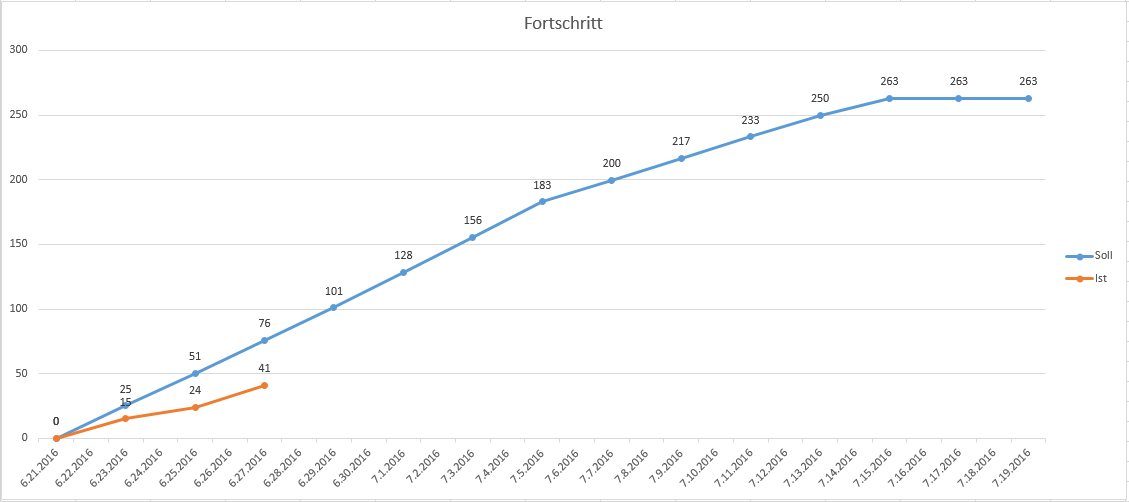
\includegraphics[width=380pt]{resourcen/week_one_diagram.PNG}
	\caption{Fortschrittsdiagramm nach Woche 1}
	\label{fig:week_one_diagram}
\end{figure}

\newpage

\section{Woche 2}
Das Ziel der Woche 2 war es, einen Graphen zu importieren und diesen, mithilfe von Mockups im Sugiyama-Algorithmus, in der Graphansicht anzuzeigen.
Dazu wurde besonders auf die zeitnahe Fertigstellung des Imports und auf die grobe Implementierung des JOANA-Graph-Plugins mit allen dazugehörigen Klassen geachtet. Zudem wurde auch in den einzelnen Phasen des Sugiyama-Algorithmus große Fortschritte gemacht und einige wurden sogar abgeschlossen. Dadurch entstand der, wie in \ref{fig:week_two_diagram} zu sehen ist, sprunghafte Anstieg des Fortschritts, welcher fast den Soll-Wert erreichte. 
\begin{figure}[!htbp]
	\centering
	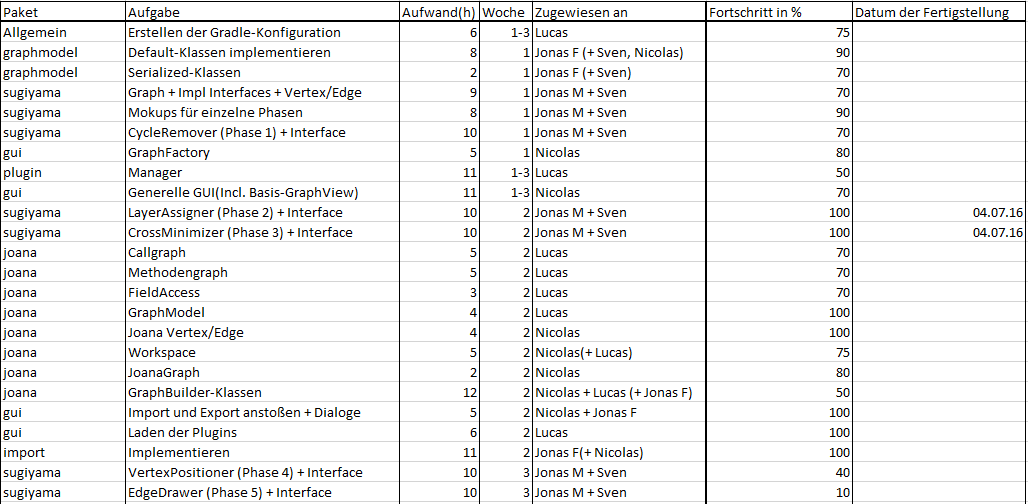
\includegraphics[width=380pt]{week_two_table.PNG}
	\caption{Implementierungsplan für Woche 1 und 2 mit Fortschritt}
	\label{fig:week_two_table}
\end{figure}
\subsection{Verzögerungen}
\label{sec:delay_week2}
Aufgrund der im Entwurf definierten Generics im GraphModel entstanden häufig sehr unschöne Stellen im Code und Inkompatibilitäten. Diese zu reparieren oder funktionsfähig zu machen war häufig der Grund für mehr oder weniger unschöne Workarounds, die teilweise viel Arbeit in Anspruch nahmen. Deshalb wurde für die folgende Woche ein großes Refactoring angesetzt, welches die Generic-Struktur im GraphModel stark vereinfachen soll.
\begin{figure}[!htbp]
	\centering
	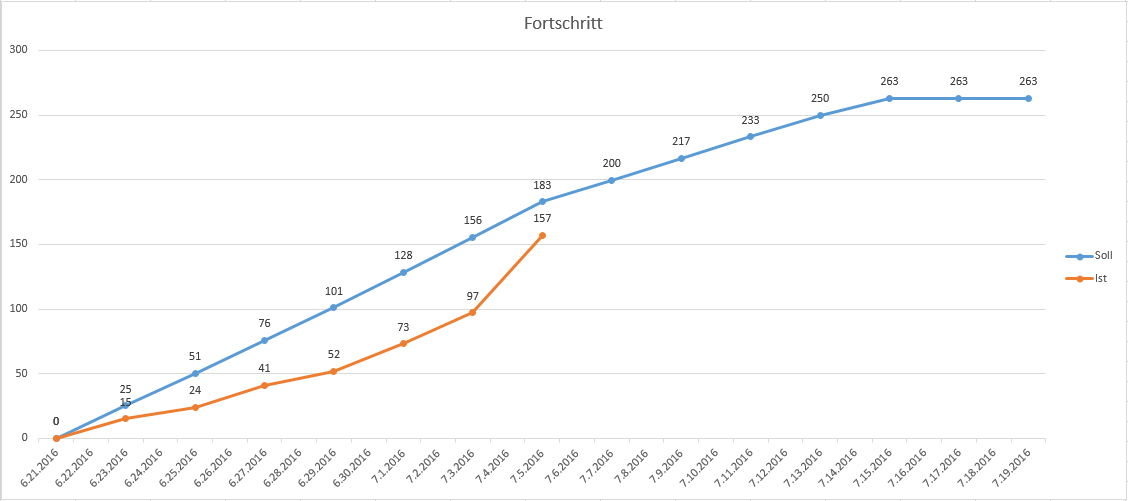
\includegraphics[width=380pt]{resourcen/week_two_diagram.PNG}
	\caption{Fortschrittsdiagramm nach Woche 2}
	\label{fig:week_two_diagram}
\end{figure}

\newpage

\section{Woche 3}
Da in Woche 3 die Oberfläche benutzbar war und man Graphen importieren und anzeigen konnte wurde neben dem in \ref{sec:delay_week2} beschriebene Refactoring, viele Bugfixes und Verbesserungen vorgenommen, die ohne eine Anzeige nicht sichtbar waren. Genau deshalb wurden in \ref{fig:week_three_table} zwar weniger Aufgaben vollständig abgeschlossen, dafür bei vielen aber ein deutlicher Fortschritt erzielt. \\
In dieser Woche wurde auch die strikte Unterteilung in die Wochen 3 und 4 aufgehoben da es für das händische Testen von anderen Aufgabenteilen an der Oberfläche anbot diese Vorzuziehen.
\begin{figure}[!htbp]
	\centering
	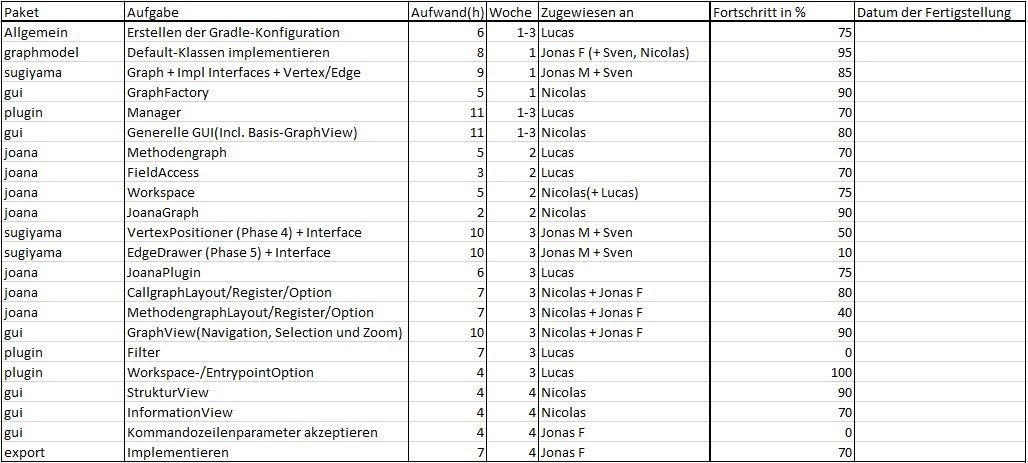
\includegraphics[width=380pt]{week_three_table.PNG}
	\caption{}
	\label{fig:week_three_table}
\end{figure}
\subsection{Verzögerungen}
Nach dem Sprint zum Ende der zweiten Woche wurde, wie in \ref{fig:week_three_diagram} zu sehen ist, zunächst weniger gearbeitet. Ab Mitte der Woche wurde aber wieder der normale Arbeitsrythmus aufgenommen und es kam zu keinen weiteren Verzögerungen.
\begin{figure}[!htbp]
	\centering
	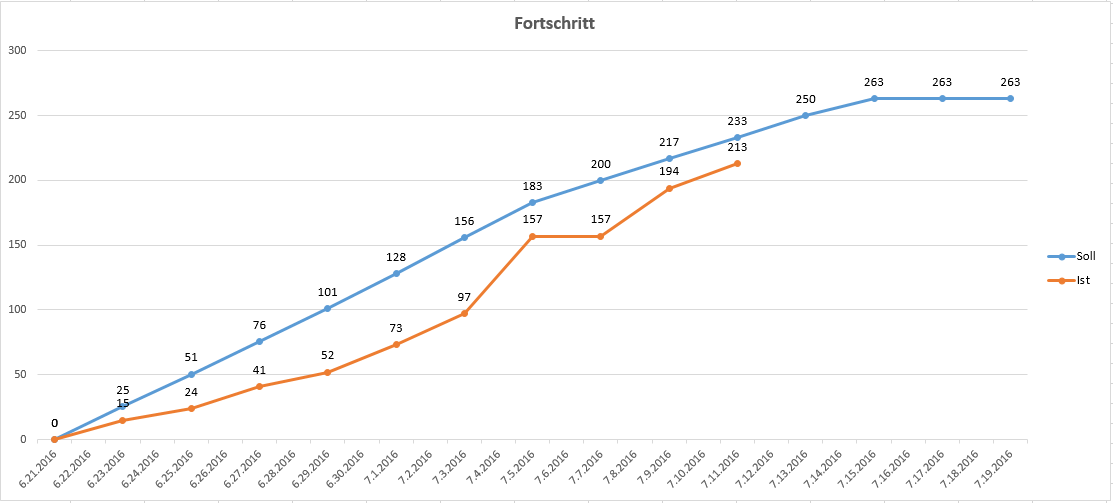
\includegraphics[width=380pt]{resourcen/week_three_diagram.PNG}
	\caption{Fortschrittsdiagramm nach Woche 3}
	\label{fig:week_three_diagram}
\end{figure}

\newpage

\section{Woche 4}
Am Ende der 4. Woche steht rückblickend fest, dass der Implementierungsplan zwar von seiner Struktur und den generellen zeitlichen Abschätzungen gut war, der Arbeitsaufwand aber in vielen Aufgabenbereichen stark unterschätzt wurde. Der Grund war häufig, das im Entwurf gemachte Designentscheidungen nicht tief genug durchdacht waren und im Laufe der Entwicklung angepasst oder komplett neu erdacht werden mussten. Solche Anpassungen haben an verschiedenen Stellen sehr viel Zeit in Anspruch genommen, welche nicht im Implementierungsplan vermerkt wurde. Diese Verzögerungen spiegeln sich besonders in der flachen Fortschrittskurve in den ersten zwei Wochen dar und haben die gesamte Entwicklung zurückgeworfen. \\
Man erkennt in \ref{fig:week_four_table} das die Ist-Kurve nach der ersten Woche fast genau so stark, manchmal sogar stärker, steigt als die Soll-Kurve. Trotzdem wurde durch die nötigen Anpassungen bedeutend mehr Zeit gebraucht als angegeben wurde. Deshalb waren auch die 16 wöchentlichen Arbeitsstunden pro Person, mit welchen die Soll-Kurve berechnet wurde, bei weitem nicht ausreichend um die Entwicklung in den vier Wochen möglichst vollständig abzuschließen. Es wurden auch die fünf Tage am Ende, die als zeitlicher Puffer eingeplant waren vollständig benötigt.
\begin{figure}[!htbp]
	\centering
	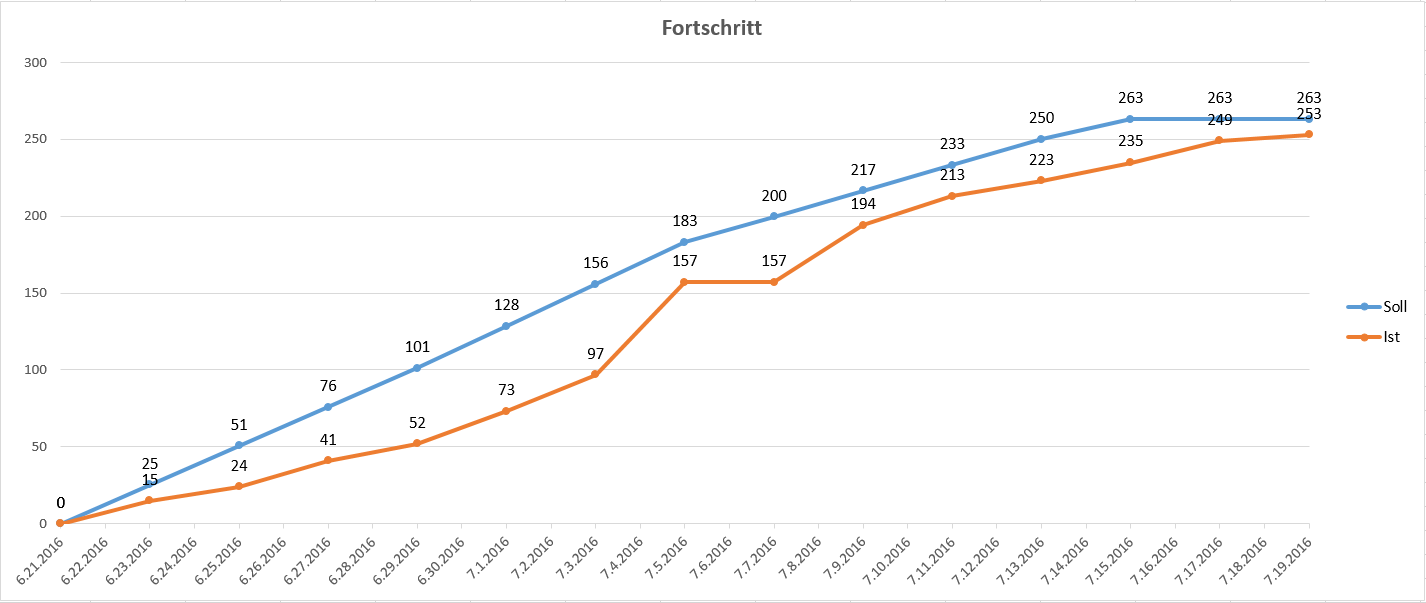
\includegraphics[width=380pt]{resourcen/week_four_diagram.PNG}
	\caption{Fortschrittsdiagramm nach Woche 4}
	\label{fig:week_four_table}
\end{figure}



\chapter{Unit Tests}
\label{ch:unittests}

\newcounter{tnr}
\newcommand\test[2]{\textbf{\arabic{tnr}}\addtocounter{tnr}{1}. & \textbf{Test:} & #1 \\ & \textbf{Aufgabe:} & #2 \\ [1ex] }

\section{Plugin}
\subsection{PluginManagerTest}
\setcounter{tnr}{1}
\begin{longtable}{llp{0.8\linewidth}}
	\test{testPluginLoad()}{Testet ob der \textit{PluginManager} alle Plugins läd.}
\end{longtable}

\section{Joana}
\subsection{JoanaGraphTest}
Importiert eine größere Anzahl von GraphML Dateien und führt mehrere Tests auf die Menge von GraphModels aus.
\setcounter{tnr}{1}
\begin{longtable}{llp{0.8\linewidth}}
	\test{test()}{Testet ob in jedem Model, die Anzahl der Kanten im CallGraph der Anzahl der MethodenGraphen entspricht.}
	\test{collapseTest()}{Testet für einen zufälligen MethodenGraphen das Kollabieren und Ausklappen von einer Knotenmenge.}
	\test{randomSymmetricCollapseTest()}{Kollabiert in einem zufälligen MethodenGraphen mehrfach Knoten, klappt sie in umgekehrter Reihenfolge wieder aus und testet auf Gleichheit zum Beginn des Tests.}
	\test{randomMixedCollapseTest()}{}
	\test{randomAssymmetricCollapseTest()}{}
\end{longtable}

\newpage

\section{Sugiyama}
\subsection{CycleRemoverTest}
\setcounter{tnr}{1}
\begin{longtable}{llp{0.8\linewidth}}
	\test{testSimpleCycle()}{Erstellt einen Testgraphen aus drei Knoten die jeweils mit einem anderen Knoten über eine gerichtete Kante verbunden sind, sodass ein Kreis entsteht. Diesen übergibt es an einen \textit{SugiyamaGraph}. Dann ruft es auf dem Cycle remover \textit{removeCycles()} mit dem \textit{SugiyamaGraph} als Parameter und testet danach ob der Graph azyklisch ist.}
	\test{testDoubleCycle()}{Erstellt einen Testgraphen aus vier Knoten und fünf gerichteten Kanten. Die Kanten sind so miteinander verknüpft, dass zwei Zykel entstehen. Ein kleiner Zykel drei Knoten beinhaltender und ein großer Zykel, der alle vier Knoten und damit auch den kleineren Zykel enthaltenden. Diesen übergibt es an einen \textit{SugiyamaGraph}. Dann ruft es auf dem Cycle remover \textit{removeCycles()} mit dem \textit{SugiyamaGraph} als Parameter und testet danach ob der Graph azyklisch ist.}
	\test{RandomGraphsTest()}{Erstellt zwanzig zufällige, zyklische \textit{SugiyamaGraphen}. Diese bestehen beim n-ten Graphen aus aus 2n Knoten und haben eine Kantendichte von $0.95^{n}$. Dann ruft es auf dem Cycle remover \textit{removeCycles()} mit dem \textit{SugiyamaGraph} als Parameter und testet danach ob der Graph azyklisch ist.}
	\test{SelfLoopTest()}{Erstellt einen Testgraphen aus einem Knoten mit einer gerichteten Kante als Selbstschleife. Diesen übergibt es an einen \textit{SugiyamaGraph}. Dann ruft es auf dem Cycle remover \textit{removeCycles()} mit dem \textit{SugiyamaGraph} als Parameter und testet danach ob diese Kante umgedreht wurde.}
\end{longtable}

\subsection{LayerAssignerTest}
\setcounter{tnr}{1}
\begin{longtable}{llp{0.8\linewidth}}
	\test{assignLayers()}{Erstellt einen azyklischen Testgraphen aus fünf Knoten, welche die korrekte Ebene für die Knoten angeben. Diese werden mit fünf Kanten verbunden. Diesen übergibt es an einen \textit{SugiyamaGraph}. Dann ruft es auf dem LayerAssigner \textit{assignLayers()} mit dem \textit{SugiyamaGraph} als Parameter und testet mithilfe der Labels, ob die Knoten den richtigen Schichten zugewiesen wurden.}
	\test{LayerAssignerTest2()}{Erstellt einen azyklischen Testgraphen aus sieben Knoten, welche die korrekte Ebene für die Knoten angeben. Diese werden mit zehn Kanten verbunden. Diesen übergibt es an einen \textit{SugiyamaGraph}. Dann ruft es auf dem  LayerAssigner \textit{assignLayers()} mit dem \textit{SugiyamaGraph} als Parameter und testet mithilfe der Labels, ob die Knoten den richtigen Schichten zugewiesen wurden.}
\end{longtable}

\subsection{CrossMinimizerTest}
\setcounter{tnr}{1}
\begin{longtable}{llp{0.8\linewidth}}
	\test{singleRandomTest()}{Erstellt einen zufälligen, zyklischen, topologisch gelayerten \textit{SugiyamaGraphen}. Diese bestehen aus 20 Knoten, die jeweils 2-8 Kanten haben. Dann ruft es auf dem CrossMinimizer \textit{minimizeCrossings()} mit dem \textit{SugiyamaGraph} als Parameter und testet danach ob die Anzahl der Kreuzungen verringert wurde oder zumindest gleich bleibt.}
	\test{randomTests()}{Erstellt 20 zufälligen, zyklischen, topologisch gelayerten \textit{SugiyamaGraphen}. Diese bestehen beim n-ten durchlauf aus ${n} + 10$ Knoten, die jeweils 3-4 Kanten haben. Dann ruft es auf dem CrossMinimizer \textit{minimizeCrossings()} mit dem \textit{SugiyamaGraph} als Parameter und testet danach ob die Anzahl der Kreuzungen verringert wurde oder zumindest gleich bleibt.}
	\test{performanceTest()}{Erstellt 20 zufälligen, zyklischen, topologisch gelayerten \textit{SugiyamaGraphen}. Diese bestehen aus 75 Knoten, die jeweils 2-8 Kanten haben. Dann ruft es auf dem CrossMinimizer \textit{minimizeCrossings()} mit dem \textit{SugiyamaGraph} als Parameter und testet danach ob die Anzahl der Kreuzungen verringert wurde oder zumindest gleich bleibt. Dabei geht es besonders um die Zeit die der Test benötigt.}
	\test{hugeTest()}{Erstellt einen zufälligen, zyklischen, topologisch gelayerten \textit{SugiyamaGraphen}. Dieser besteht aus 250 Knoten, die jeweils 2-6 Kanten haben. Dann ruft es auf dem CrossMinimizer \textit{minimizeCrossings()} mit dem \textit{SugiyamaGraph} als Parameter und testet danach ob die Anzahl der Kreuzungen verringert wurde oder zumindest gleich bleibt. Dabei geht es besonders um die Zeit die der Test benötigt.}
\end{longtable}

\subsection{VertexPositionerTest}
\setcounter{tnr}{1}
\begin{longtable}{llp{0.8\linewidth}}
	\test{positionVertices()}{Testet nichts...?!}
\end{longtable}

\subsection{EdgeDrawerTest}
\setcounter{tnr}{1}
\begin{longtable}{llp{0.8\linewidth}}
	\test{compileTest()}{Testet nichts...?!}
\end{longtable}

\subsection{SugiyamaLayoutAlgorithmTest}
Für jeden Test wird ein kompletter Sugiyama-Layout-Algorithmus angewendet.
\setcounter{tnr}{1}
\begin{longtable}{llp{0.8\linewidth}}
	\test{testSmallGraph()}{Testet für einen Graphen mit vier Knoten und fünf Kanten ob der gesamte Algorithmus ohne Fehler durchläuft.}
	\test{testRandomGraph()}{Testet für drei zufällige Graphen ob der gesamte Algorithmus ohne Fehler durchläuft.}
\end{longtable}

\clearpage

%\bibliography{referenzen}
\end{document}
